%TELLING TIME \\& ELAPSED TIME - WORKSHEET 0 (IN-CLASS INSTRUCTION)
\documentclass[12pt, letterpaper, fleqn]{article}

% ----------------------------------------------------------
% PACKAGES
% ----------------------------------------------------------
\usepackage{graphicx}
\usepackage{xcolor}
\usepackage[most]{tcolorbox}
\usepackage{amsmath, amssymb}
\usepackage{fancyhdr}
\usepackage[utf8]{inputenc}
\usepackage[T1]{fontenc}
\usepackage{enumitem}
\usepackage{geometry}
\usepackage{tikz}
\usepackage{needspace}
\usepackage{multicol}

\usetikzlibrary{arrows.meta, calc, shapes.geometric}

% ----------------------------------------------------------
% PAGE SETUP
% ----------------------------------------------------------
\usepackage{times}
\geometry{letterpaper, top=1.25in, bottom=1.25in, marginpar=0.5in}

% ----------------------------------------------------------
% HEADER / FOOTER
% ----------------------------------------------------------
\newcommand{\logowidth}{3cm}
\setlength{\headheight}{20pt}
\setlength{\footskip}{40pt}

\pagestyle{fancy}
\fancyhf{}
\fancyhead[C]{\small\bfseries Telling Time \\& Elapsed Time}
\fancyfoot[L]{\raisebox{2pt}{
\includegraphics[width=\logowidth]{../kss.png}}}
\fancyfoot[C]{\thepage}
\fancyfoot[R]{3.18.0}

\renewcommand{\footrulewidth}{0.2pt}

% ----------------------------------------------------------
% THEME COLOR
% ----------------------------------------------------------
\definecolor{customteal}{HTML}{2fbdb9}

% ----------------------------------------------------------
% HELPER MACROS
% ----------------------------------------------------------
\newcommand{\blank}{\underline{\hspace{2.2cm}}}
\newcommand{\blanklong}{\underline{\hspace{6.5cm}}}
\newcommand{\blankshorter}{\underline{\hspace{1.5cm}}}

% ----------------------------------------------------------
% DOCUMENT
% ----------------------------------------------------------
\begin{document}

\textbf{Name:} \underline{\hspace{5cm}}
\hfill
\textbf{Date:} \underline{\hspace{3cm}}\\

\begin{tcolorbox}[colback=customteal!20]
    \large\textcolor{black}{\textbf{Telling Time \& Elapsed Time}}
\end{tcolorbox}

\vspace{3mm}
\noindent
An **analog clock** has:
\begin{itemize}
    \item A short hand to show the **hour**.
    \item A long hand to show the **minute**.
\end{itemize}
**Elapsed time** is the amount of time that passes from a start time to an end time.

\begin{center}
\begin{tikzpicture}[scale=0.9]
\draw[thick] (0,0) circle (1.8cm);
\foreach \angle [count=\label] in {60,30,0,-30,-60,-90,-120,-150,-180,-210,-240,-270} {
  \draw (\angle:1.6cm) -- (\angle:1.8cm);
  \node at (\angle:1.3cm) {\small\textsf{\label}};
}
% Hands for 10:10
\draw[line width=1.5pt, -latex] (0,0) -- (60:1.2cm); % Minute hand
\draw[line width=2.5pt, -latex] (0,0) -- (300:0.8cm); % Hour hand
\fill (0,0) circle (2pt);
\end{tikzpicture}
\end{center}

\newpage
\begin{tcolorbox}[colback=customteal!20]
    \large\textcolor{black}{\textbf{Guided Practice}}
\end{tcolorbox}

\vspace{5mm}
\begin{enumerate}[itemsep=3cm, leftmargin=0.6cm]
\item What time is shown on the clock in the picture above?
\\
Time: \blank : \blank

\item School begins at 8:15 AM and recess starts at 9:00 AM. How many minutes of elapsed class time are there?
\\
Calculation space: \vspace{2cm}
\\
Answer: \blank minutes
\end{enumerate}

\end{document}
